\documentclass[a4paper,12pt]{article}
%管理引用参考文献
\usepackage{cite}
%指定输入文件的编码格式
\usepackage[utf8]{inputenc}
%中文排版支持
\usepackage{ctex}
%数学公式支持
\usepackage{amsmath}
%超链接与颜色支持
\usepackage{hyperref}
\usepackage{xcolor}
\usepackage[a4paper, margin=1in]{geometry}
\usepackage{graphicx}
\usepackage{float}
\usepackage{caption}
\usepackage{booktabs}
\usepackage{pgfpages}
\usepackage{subcaption}
\usepackage{xcolor}
\usepackage{array}
\usepackage{dcolumn}
\usepackage{caption}
\usepackage{tcolorbox}




% 设置引用颜色
\hypersetup{
    colorlinks=true,       % 启用链接的颜色
    linkcolor=blue,        % 内部链接的颜色(例如目录链接)
    citecolor=red,         % 引用文献的颜色
    urlcolor=blue          % URL链接的颜色
}
\usepackage{cite}

\title{因果推断课程报告}
\author{田晨楷 2211333}
\date{\today}

\begin{document}

\maketitle

\section{引言}
\subsection{背景介绍}
随着全球城市化进程的加速,环境污染问题已成为各国政府和社会各界关注的焦点。城市化带来了经济发展和生活水平的提升,但同时也导致了空气质量恶化、水体污染和生态破坏等一系列环境问题。根据统计数据,中国在过去几十年中经历了快速的城市化,许多城市面临着严重的环境污染挑战,尤其是在工业化程度较高的地区。

为应对环境污染和可持续发展的挑战,中国政府提出了智慧城市建设(Smart City Construction, SCC)政策。智慧城市通过整合信息技术、物联网和大数据等现代科技手段,旨在优化城市管理、提升公共服务效率,并实现资源的高效利用。自2013年起,中国开始实施智慧城市试点政策,首批和第二批试点城市于2013年公布,第三批试点城市于2015年公布。本研究把智慧城市建设政策视作一个准自然实验。这样的外生政策冲击,为我们提供了因果推断的机会。


\subsection{研究目的}
本研究旨在通过因果推断的方法,系统分析智慧城市建设政策对中国城市污染排放的影响。具体而言,我们将利用双重差分模型(Difference-in-Difference, DiD)作为基准模型分析,再通过设计新的倾向匹配得分(Propensity Score Matching, PSM)方法,并引入机器学习算法提高稳健性和识别异质性,不断挖掘政策实施中的因果效应,探讨智慧城市建设如何对城市污染排放产生影响。研究的核心问题包括:

\begin{itemize}
    \item 智能城市政策是否有效地降低了城市的污染排放?
    \item 这种影响在不同城市和地区之间是否存在异质性?
\end{itemize}

通过对这些问题的深入探讨,本研究希望为政策制定者提供科学依据,推动智慧城市建设的进一步发展,从而实现可持续的城市发展目标。

\subsection{研究路线}
在本研究旨在全面评估智慧城市建设政策对城市污染排放的影响。

首先,我们通过基准回归模型来估计智慧城市政策对污染排放的直接影响。为了确保我们的估计结果不是由于其他未观测因素的干扰,我们进行了平行趋势检验。这一步骤验证了在智慧城市建设政策实施之前,处理组和对照组的污染排放趋势是否相似,这是双重差分模型有效性的关键前提。接着,我们通过安慰剂检验来进一步验证模型的稳健性。这一检验通过随机分配处理效应,帮助我们确认观察到的政策效应不是由随机因素引起的。此外,我们运用了Bacon分解方法来深入分析不同因素对估计结果的具体贡献。

为了解决可能的样本选择偏差问题,我们采用了针对于\textbf{面板数据}的倾向得分匹配与双重差分相结合的方法(PSM-DiD)。这种方法通过匹配处理组和对照组的倾向得分,减少了由于个体特征差异带来的估计偏差,并且不存在\textbf{自匹配}的问题,从而提高了估计的准确性。

在稳健性检验方面,我们替换因变量重新进行了估计,并应用了双重去偏机器学习算法。这些方法有助于确保我们的估计结果在不同模型设定下依然稳健。

最后,我们通过因果森林的机器学习算法进行了异质性分析,探讨了不同城市特征和区域差异对智慧城市建设政策效果的异质性。这有助于我们理解政策在不同环境下的适用性和效果差异。


\subsection{研究框架}

图\ref{fig:frame}展示了本研究的框架。

\begin{figure}[H]
    \centering
    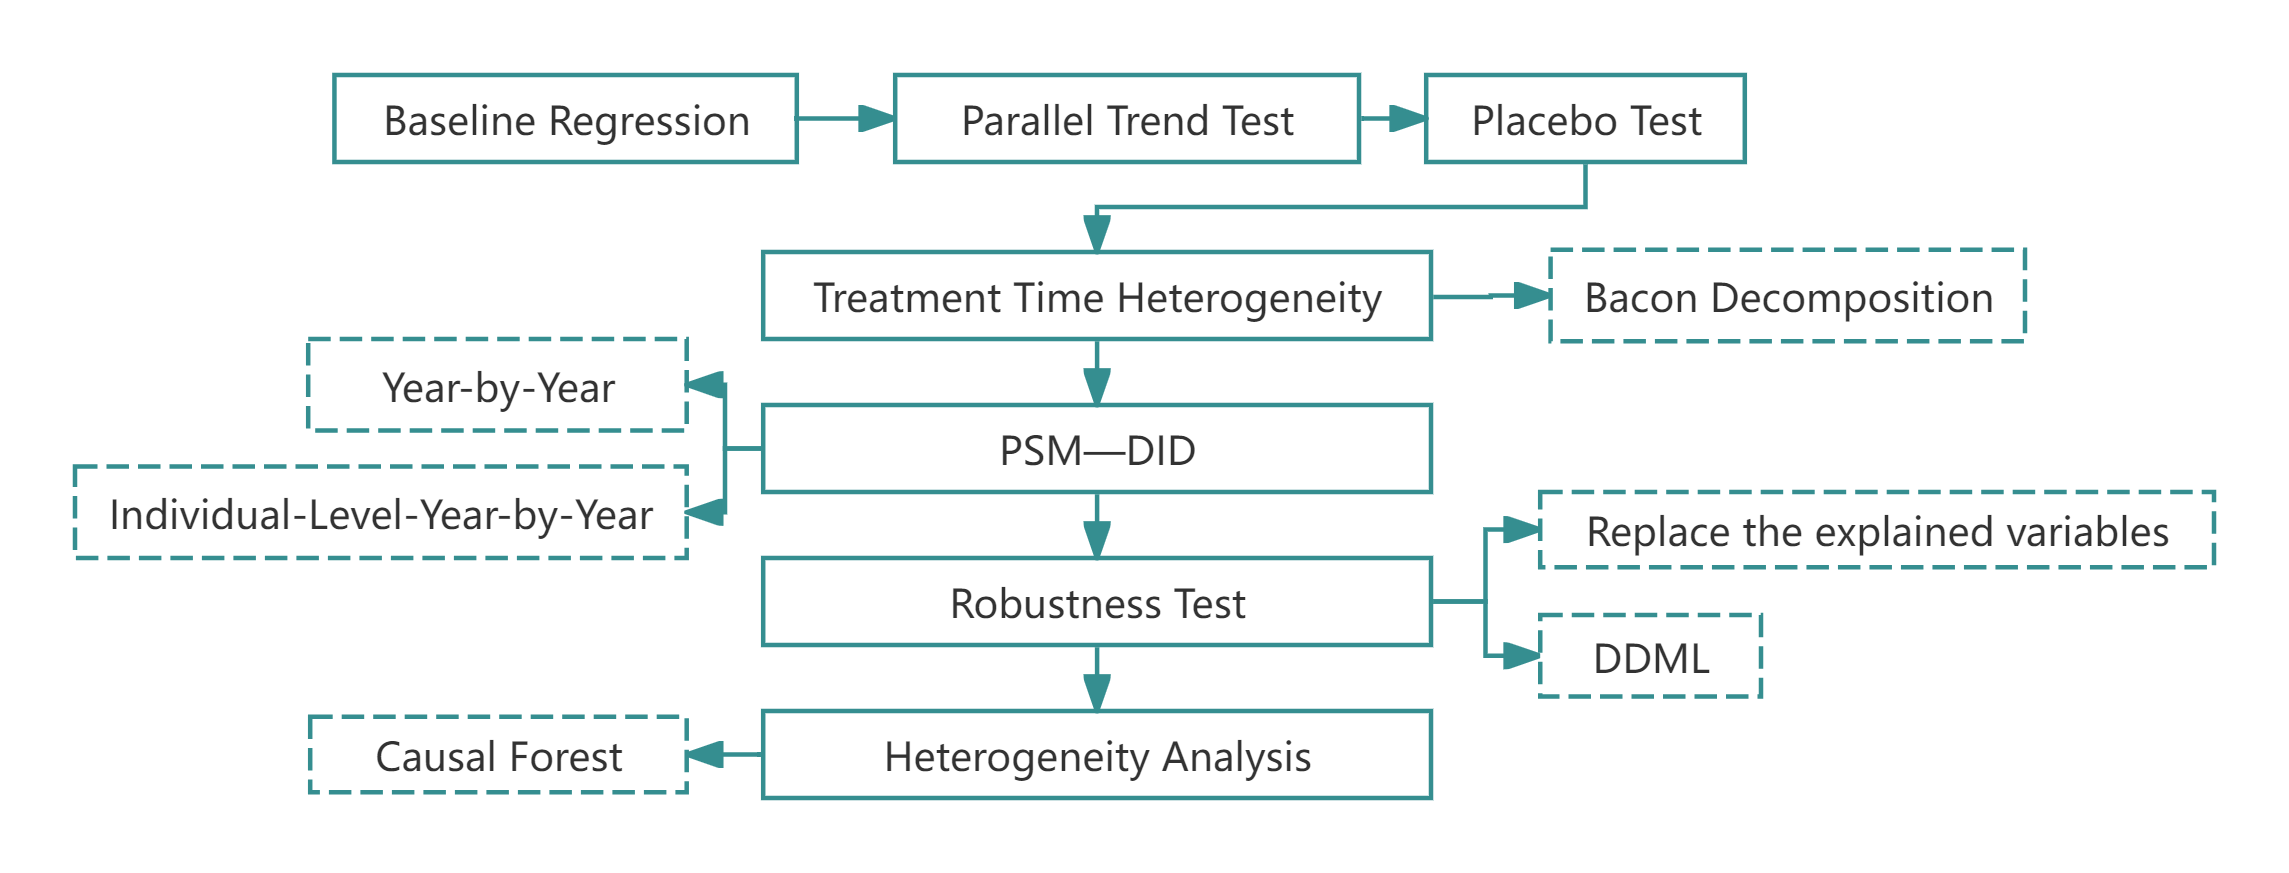
\includegraphics[width=\textwidth]{framework.jpg}
    \caption{框架图}
    \label{fig:frame}  
\end{figure}


\section{数据和变量}

\subsection{数据集}
本研究使用的数据集来源于《中国城市统计年鉴》,是涵盖了298个中国城市的平衡面板数据集。其中,119个城市被选为智慧城市试点。数据集包含了从2003年到2019年的5066个观测值。这些数据为研究提供了丰富的实证基础,使得我们能够深入分析智慧城市建设政策对城市污染排放的影响。

图\ref{fig:pilot}展示了298个城市接受试点的时间图。我们可以看到,数据集中存在充足的空白对照组,是PSM-DiD模型匹配环节的重要基础。

\begin{figure}[H]
    \centering
    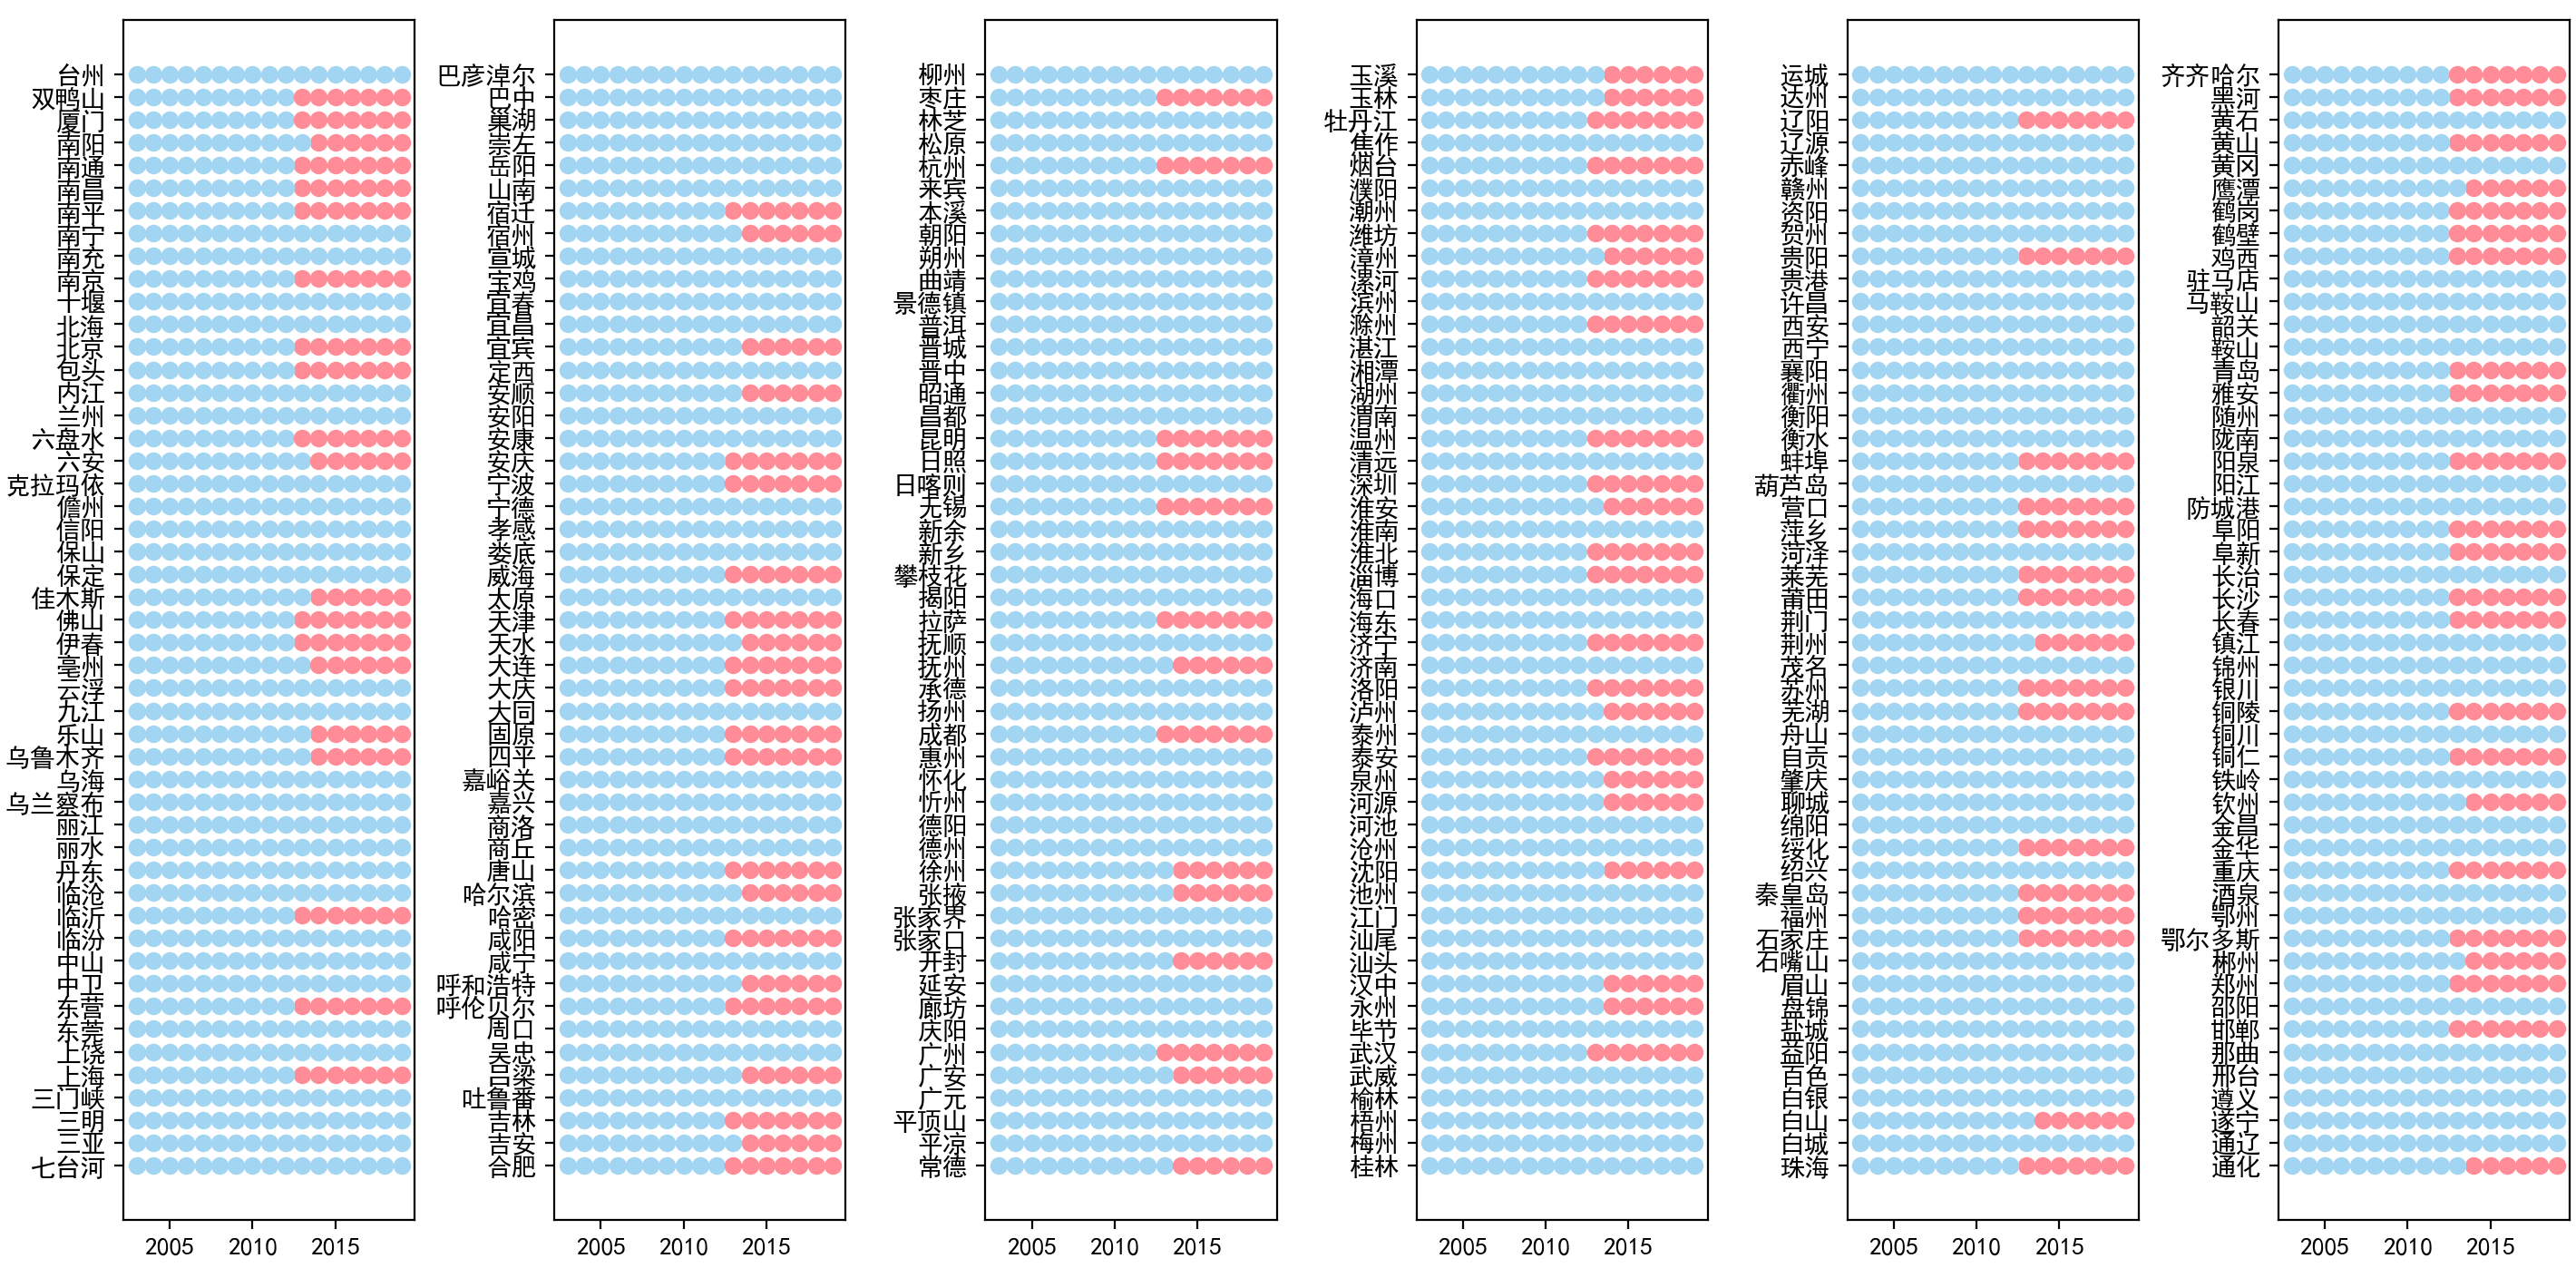
\includegraphics[width=\textwidth]{pilot.jpg}  
    \caption{城市试点时间图}
    \label{fig:pilot}  
\end{figure}


\subsection{变量定义}

\subsubsection{因变量:城市污染排放}

熵权法是一种客观赋权的综合评价方法,能够科学地反映各污染指标的相对重要性,从而为城市污染排放的量化提供依据。本研究参考\cite{wang2024beautifying},通过熵权法综合评估工业废水、二氧化硫和工业烟尘的排放情况,构建城市污染排放作为本研究的因变量。熵权法的具体步骤如下:

1.进行标准化处理:

$$
    X_{i j t}^{\prime}=\frac{x_{i j t}-\min \left(x_{m j t}\right)}{\max \left(x_{m j t}\right)-\min \left(x_{m j t}\right)}
$$


2.对于第$j$个污染指标,计算第$i$个城市在时间$t$的相对比例:

$$
P_{i j t}=\frac{X_{i j t}^{\prime}}{\sum_{i=1}^m X_{i j t}^{\prime}}\left(0 \leq P_{i j t} \leq 1\right)
$$

3.计算第$j$个污染指标在时间$t$的熵$e_{jt}$:

$$
e_{j t}=-\frac{1}{\ln m} \sum_{i=1}^m P_{i j t} \ln P_{i j t}\left(0 \leq e_{j t} \leq 1\right)
$$

4.计算赋予第$j$个污染指标在时间$t$的权重$W_{jt}$:

$$
W_{j t}=\frac{g_{j t}}{\sum_{j=1}^n g_{j t}}, g_{j t}=1-e_{j t}\left(0 \leq g_{j t} \leq 1, W_1+W_2+\bullet \bullet \bullet +W_j=1\right)
$$

5.获得第$i$个城市在时间$t$的综合污染指标:

$$
Poll_{i t}=\sum_{j=1}^n W_{j t} \times P_{i j t}
$$



\subsubsection{自变量:智慧城市政策}

智慧城市政策(SCC)被定义为智慧城市(smart)与政策实施时间(post)两个虚拟变量的交互项。具体而言,如果一个城市被设定为智慧城市,则$smart$取值为1,作为处理组;否则取值为0,作为对照组。时间虚拟变量$post$在SCC实施前后分别取值为0和1,以标识政策实施的时间节点。

$$
SCC = smart \times post
$$

\subsubsection{控制变量}

为了更准确地评估智慧城市政策对污染排放的影响,并排除其他潜在混杂因素的干扰,本研究参考\cite{wang2024beautifying}纳入了多个控制变量:

\begin{table}[H]
\centering
\scalebox{0.85}{
\begin{tabular}{ccp{6cm}}
\toprule
 & Variable & Measurement \\
\midrule

Control Variable & ln\_GDP & Natural logarithm of GDP \\
 & government\_intervention & Ratio of government fiscal
expenditure to GDP \\
 & urbanization\_level & Ratio of population to
registered population \\
 & financial\_development & Ratio of outstanding loans
of financial institutions to
GDP \\
 & population\_density & Ratio of registered urban
population to administrative area \\
 & education\_level & Natural logarithm of the
number of college students \\
\bottomrule
\end{tabular}
}
\end{table}

\subsection{描述性统计}

\subsubsection{相关系数矩阵}
图\ref{fig:Correlation}展示了主要变量之间的相关系数。变量之间存在小但显著的相关系数,表明不存在多重共线性。
\begin{figure}[H]
    \centering
    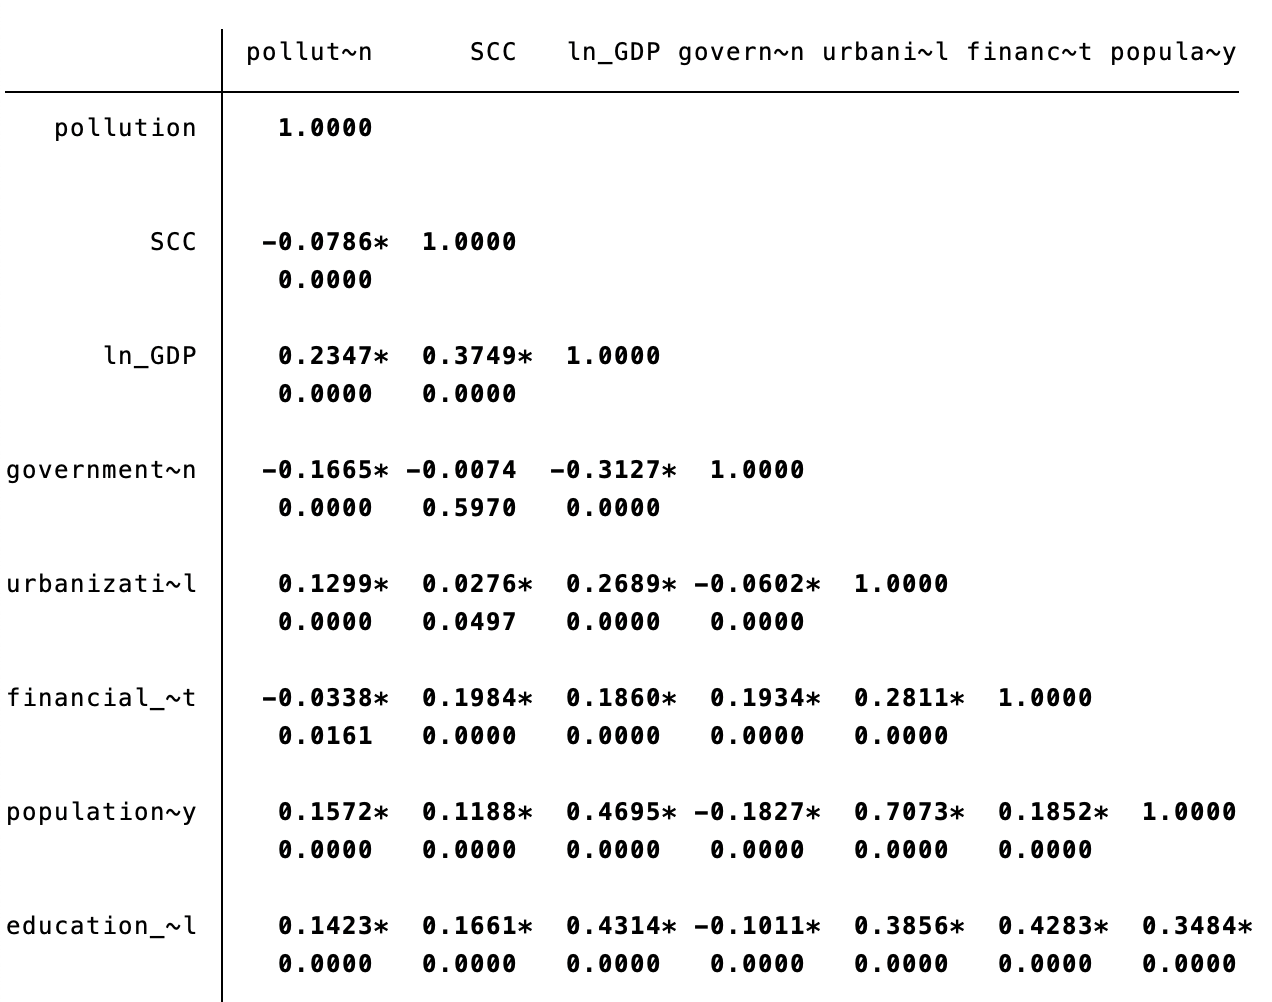
\includegraphics[width=0.7\textwidth]{Correlation.png}
    \caption{相关系数矩阵}
    \label{fig:Correlation}  
\end{figure}


\subsubsection{Jarque-Bera检验}

本研究对主要变量进行了Jarque-Bera检验。图\ref{fig:JB}展示了检验结果,绝大多数检验的p值为0,拒绝数据呈正态分布的原假设。鉴于样本量较大,偏离正态分布不太可能对回归结果产生显著影响。

\begin{figure}[H]
    \centering
    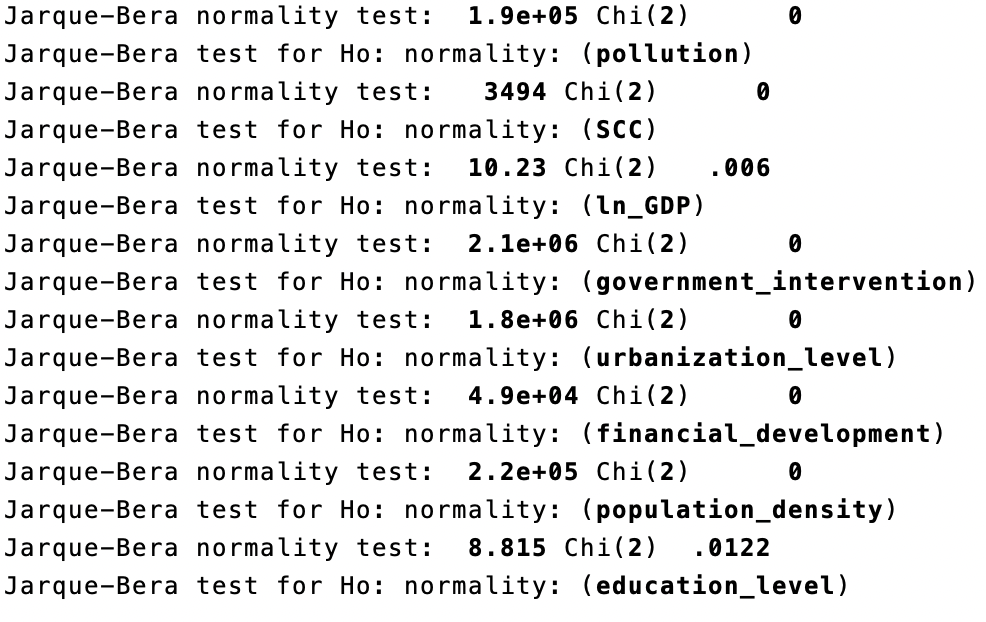
\includegraphics[width=0.6\textwidth]{JB.png} 
    \caption{正态性检验结果}
    \label{fig:JB}  
\end{figure}

\section{实证分析}

\subsection{基准回归}

我们采用以下回归模型进行分析:

$$
Poll_{i t}=\beta_0+\beta_1 SSC_{i t}+\beta_2 Control_{i t}+ u_i+ \eta_t+\epsilon_{i t}
$$

其中:$i$和$t$分别代表城市和时间。$\beta_1$捕捉了智慧城市政策对城市污染排放的影响。$u_i$和$\eta_t$分别代表城市和时间的固定效应,$\epsilon_{it}$是随机扰动项。

多期DiD模型评估智慧城市政策对城市污染水平的影响的结果如下\ref{tab:BR}。模型中包括城市和年份的固定效应,以控制不随时间变化的城市特有因素和全国性的时间趋势。

\begin{table}[H]
\centering
\resizebox{0.7\textwidth}{!}{
\begin{tabular}{lcccccc}
& \textbf{Without controls} & \textbf{With controls} \\

\hline
\textbf{SCC}                &      -0.200***&      -0.198***\\
                    &    (0.0725)   &    (0.0758)   \\
government\_intervention&               &     -0.0333   \\
                    &               &    (0.0954)   \\
urbanization\_level  &               &       0.144   \\
                    &               &     (0.152)   \\

financial\_development&               &      0.0123   \\
                    &               &    (0.0475)   \\

population\_density  &               &       0.861   \\
                    &               &     (7.212)   \\

education\_level     &               &     -0.0329   \\
                    &               &    (0.0203)   \\

Constant            &      0.0911***&      -3.141*  \\
                    &    (0.0342)   &     (1.718)   \\
\hline
Observations        &        5066   &        5066   \\
$R^2$                 &       0.322   &       0.328   \\
Year FE & Y & Y\\
City FE & Y & Y\\
\hline
\end{tabular}
}
\caption{基准回归结果}
\label{tab:BR}
\end{table}

包含和不包含控制变量时,智慧城市政策(SCC)的估计系数均显著为负,表明智慧城市政策会显著地降低城市污染水平。

\subsection{平行趋势检验}
DiD模型的有效性依赖于处理组和对照组在政策实施前具有相似的趋势。因此,我们采用如下动态回归模型进行平行趋势检验:

$$
Poll_{i t}=\beta_0+\sum_{t=2}^{t=5}\alpha_{t} Pre_{i t}+ \sum_{t=0}^{t=5} \beta_{t}Post_{it} + \gamma Control_{i t}+ u_i+ \eta_t+\epsilon_{i t}
$$

为了避免完全共线性,我们将$Pre_1$剔除。

图\ref{fig:Parallel Trend}展示了平行趋势检验的结果。从图中可以看出,在智慧城市政策实施之前,处理组和对照组的动态效应估计值大致在0附近波动,不显著异于0,这表明在政策实施前,处理组和对照组之间没有显著的趋势差异,符合平行趋势假设。在政策实施后,动态效应估计值呈现下降趋势,显著异于0,这表明智慧城市政策对降低污染排放有显著效果。

\begin{figure}[H]
    \centering
    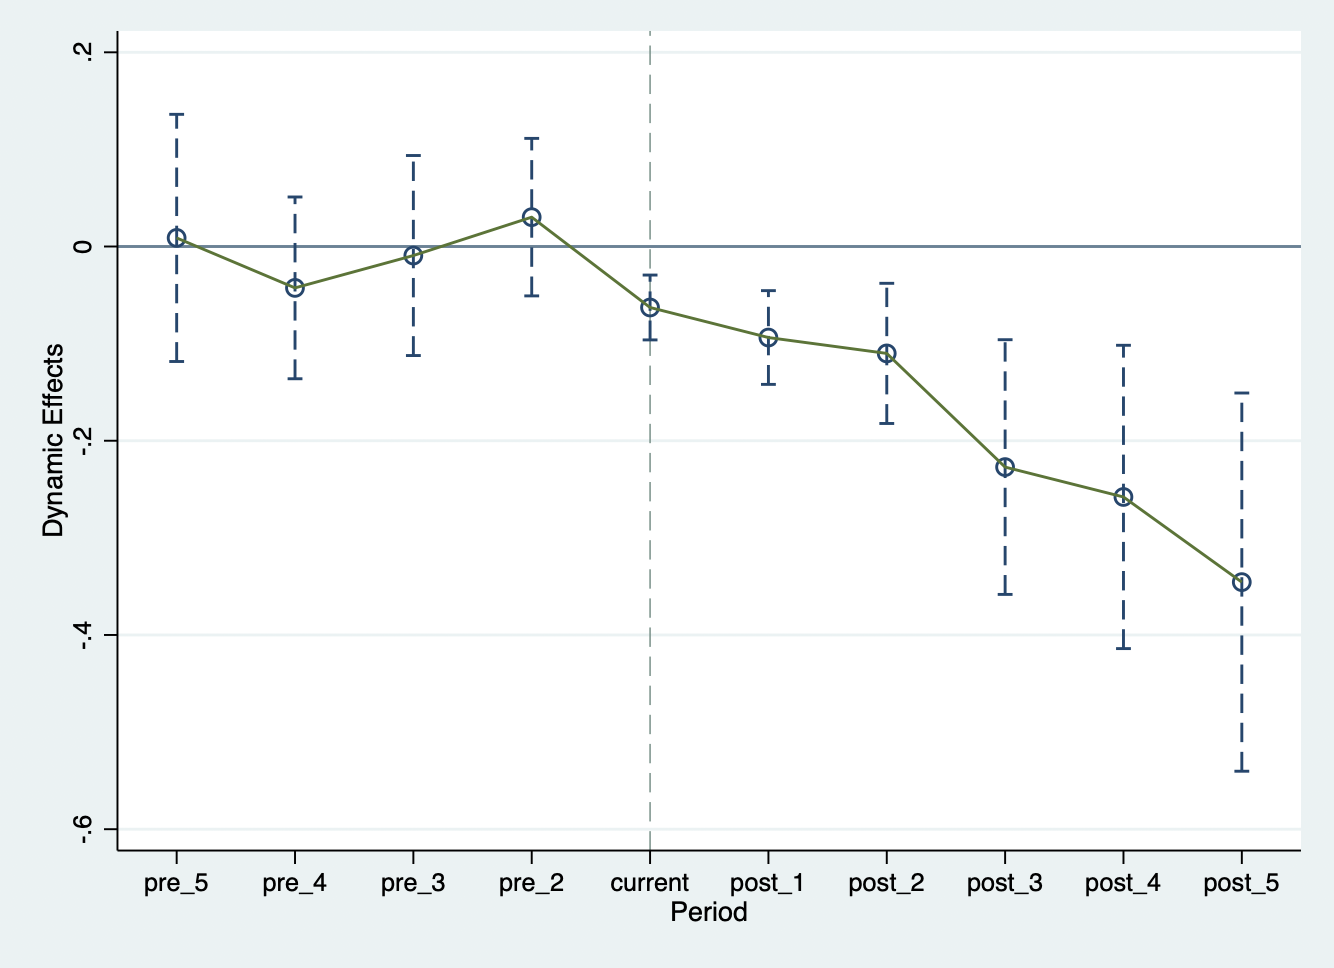
\includegraphics[width=0.8\textwidth]{Parallel Trend.png} 
    \caption{平行趋势检验结果}
    \label{fig:Parallel Trend}  
\end{figure}



\subsection{安慰剂检验}
考虑到估计结果可能会受到其他随机因素的干扰,本研究通过随机生成伪处理组城市和虚拟时间变量来进行安慰剂检验,通过重复进行回归分析,观察估计系数的分布情况。若大部分估计系数集中在0附近,且p值大于0.1,则表明原始结果的显著性不受随机因素影响。

图\ref{fig:Placebo}展示了安慰剂检验的结果。结果表明:估计系数主要集中在0附近,大多数回归的p值都超过了0.1,表明大部分结果不显著。

\begin{figure}[H]
    \centering
    \caption{不同重复次数的安慰剂检验}
    \begin{subfigure}[b]{0.45\textwidth}
        \centering
        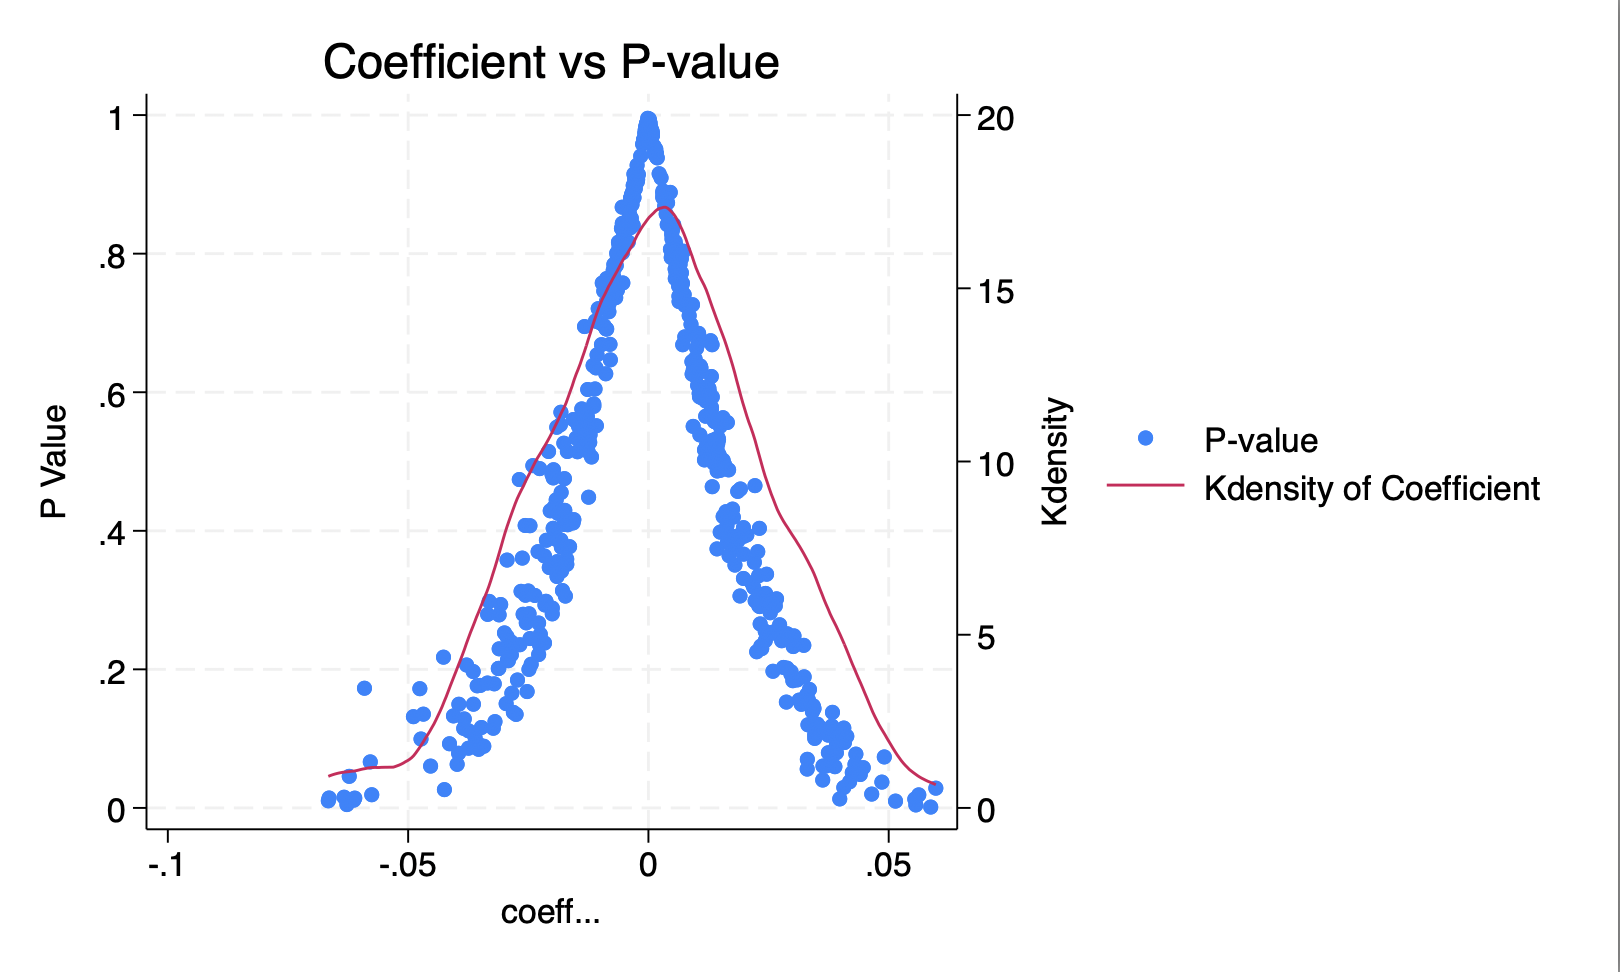
\includegraphics[width=\textwidth]{500.png}
        \caption{500 repititions}
        \label{fig:Placebo1}
    \end{subfigure}
    \hfill
    \begin{subfigure}[b]{0.45\textwidth}
        \centering
        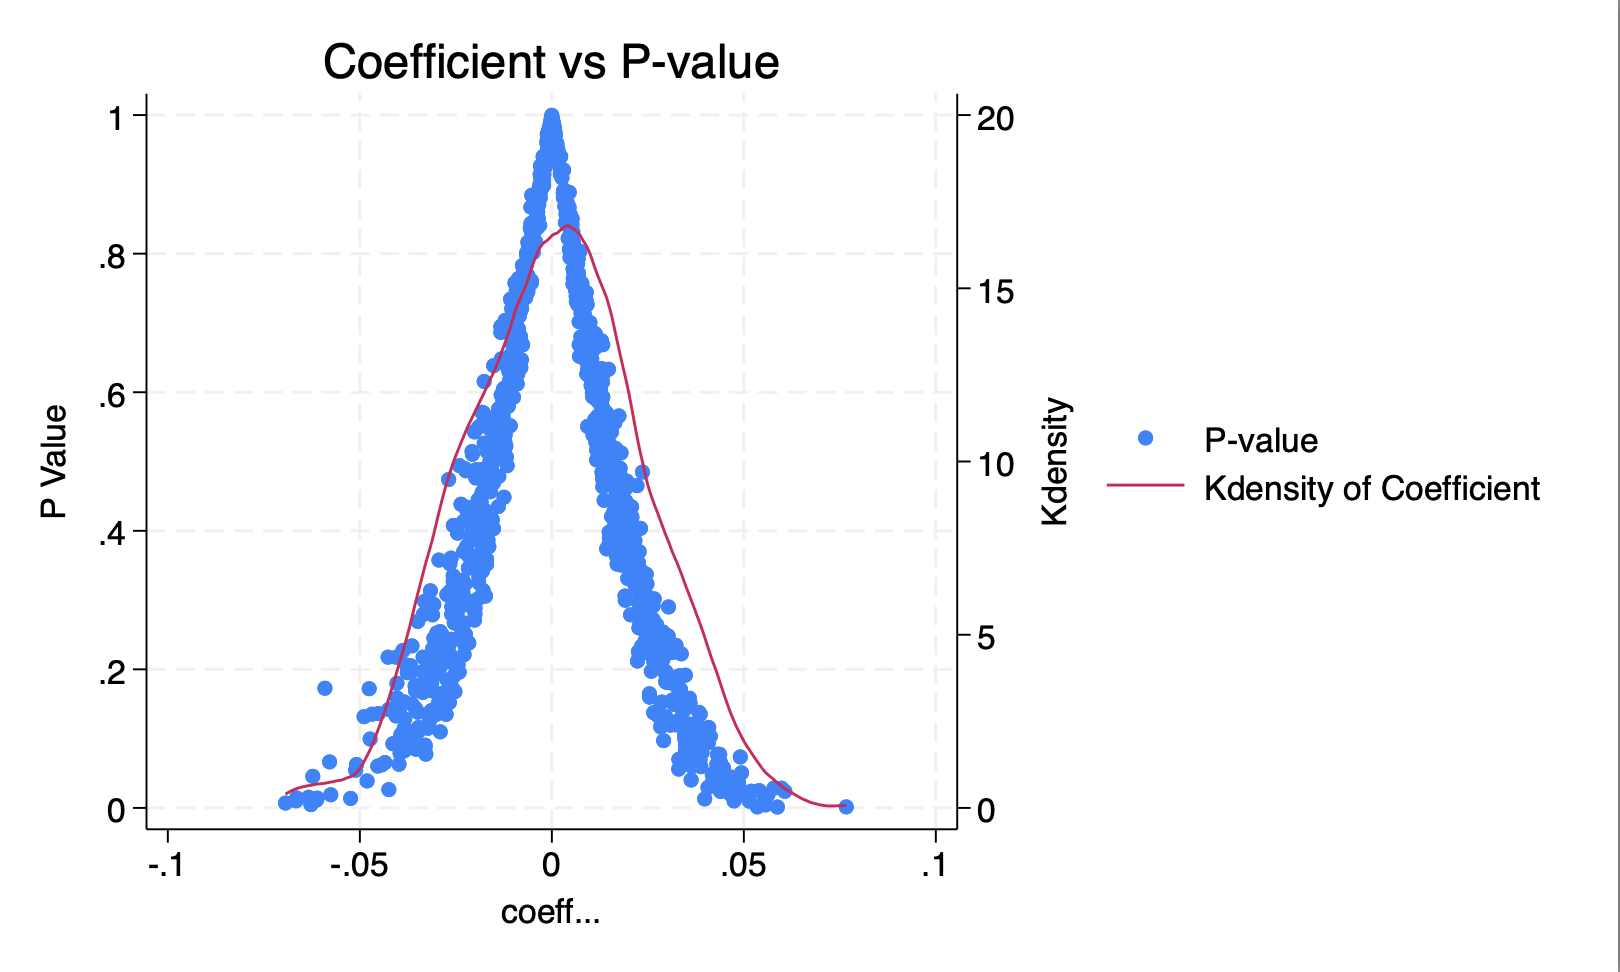
\includegraphics[width=\textwidth]{1000.png}
        \caption{1000 repititions}
        \label{fig:Placebo2}
    \end{subfigure}
    \label{fig:Placebo}
\end{figure}

\subsection{Bacon分解}

为了分析处理效果在不同时间组(Timing Groups)或不同处理时机下的异质性,我们进行了
Bacon分解,将总的因果效应分解为不同组别的贡献。

$$
\begin{gathered}
\sum_t s_t+\sum_{e t \neq u t} \sum_{l t>e t}\left(s_{e t}+s_{l t}\right)=1 \\
\hat{\beta}^{D I D}=\sum_t s_t \hat{\beta}_{t, u t}^{D I D}+\sum_{e t \neq u t} \sum_{l t>e t}\left(s_{e t} \hat{\beta}_{e t, y u t}^{D I D}+s_{l t} \hat{\beta}_{l t, e t}^{D I D}\right)
\end{gathered}
$$

图\ref{fig:Bacon Decomposition1}和图\ref{fig:Bacon Decomposition2}展示了Bacon分解的结果。

\begin{figure}[H]
    \centering
    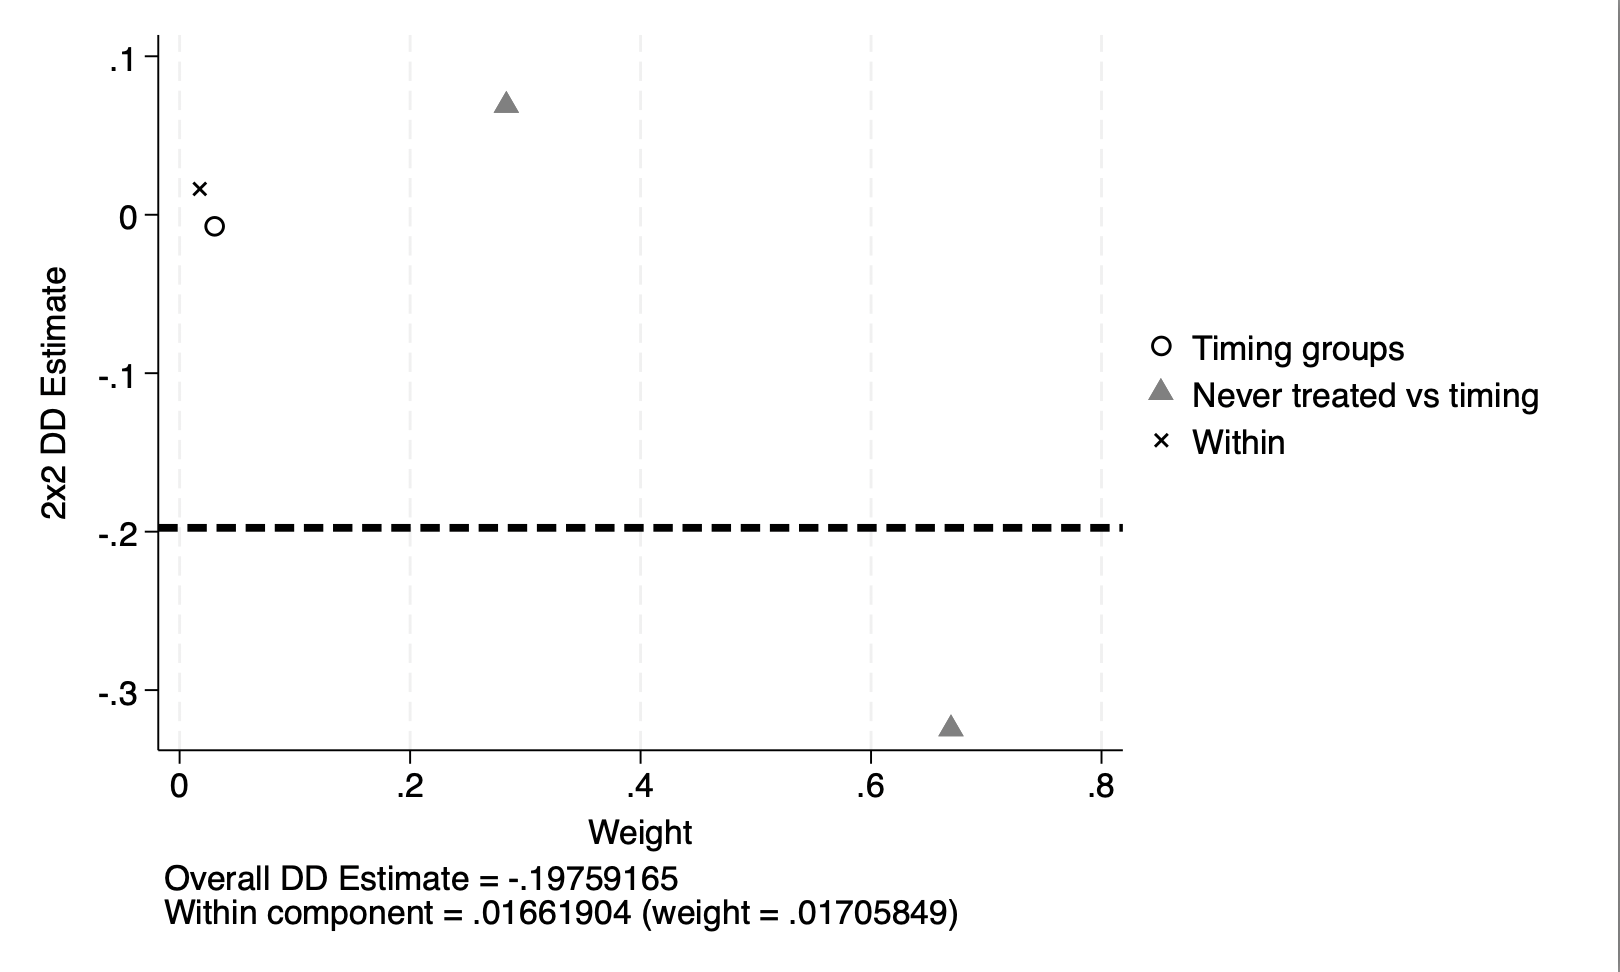
\includegraphics[width=0.8\textwidth]{Bacon1.png}
    \caption{Bacon分解结果1}
    \label{fig:Bacon Decomposition1}  
\end{figure}

\begin{figure}[H]
    \centering
    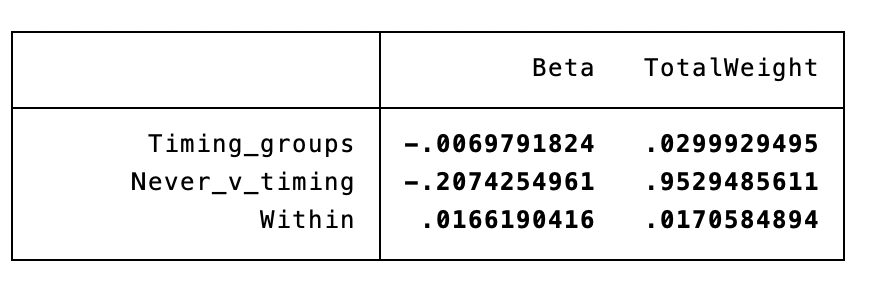
\includegraphics[width=0.8\textwidth]{Bacon2.png}
    \caption{Bacon分解结果2}
    \label{fig:Bacon Decomposition2}  
\end{figure}

Timing\_groups 指的是根据不同处理时机(即处理开始的时间或处理的持续时间)划分的群组。
时机组别在总体效应中占比约为3.0\%。这意味着这些时机组别对总体因果效应的贡献较小。

Never\_v\_timing 表示从未接受处理的群组(对照组)与接受处理的不同时机组别之间的比较。具体来说,这部分反映了从未处理群组与所有处理群组(无论处理时机如何)的效应差异。
这部分在总体效应中的权重占比约为95.3\%。这是分解结果中占比最高的部分,说明从未处理与处理群组之间的差异是总体因果效应的主要驱动因素。

Within表示在各个处理时机组别内部的效应差异。这部分关注的是在同一时机组别内,不同个体之间或不同处理强度下的效应差异。这部分在总体效应中的权重占比约为1.7\%,说明组内效应对总体因果效应的贡献极小。



\subsection{PSM-DiD}

考虑到智慧城市试点可能存在的样本选择偏差,本研究拟采用PSM-DiD模型进行估计,以减少选择偏差对结果的影响。利用数据集存在大量空白对照组的特点,我们采用两种针对\textbf{面板数据}的匹配方法。

\begin{itemize}
    \item 逐年匹配方法(Year-by-Year Matching)
\end{itemize}

逐年匹配的思想是:在同一年份基于处理状态逐年进行匹配。具体步骤如下:首先,计算每个城市每年的倾向得分;然后,对于每一年,根据倾向得分将处理组与最相似的对照组进行匹配。通过逐年匹配,确保在每个时间点上处理组和对照组尽可能相似,减少随时间变化的偏差。

\begin{itemize}
    \item 个体层面逐年匹配方法(Individual-Level Year-by-Year Matching)
\end{itemize}

此外,我们设计了一种适用于面板数据的匹配方法:个体层面逐年匹配。这种方法扩展了逐年匹配,将每个单位在所有年份的倾向得分视为多维向量,根据倾向得分向量的整体相似性进行匹配。具体步骤如下:首先,计算所有城市每年的倾向得分并构建多维向量;然后,对于每个处理组,计算其倾向得分向量与对照组倾向得分向量之间的欧几里得距离;最后基于倾向得分向量,将每个处理组中的城市与距离最小的对照组中的城市进行匹配。

匹配结果如下\ref{tab:code}:

\begin{table}[H]
    \centering
    \begin{tabular}{ccc}
\toprule
& \textbf{Treated Group} & \textbf{Control Group}\\
\midrule
0 & 440300 & 370100 \\
1 & 350200 & 370100 \\
2 & 440400 & 321100 \\
3 & 440600 & 320400 \\
4 & 371200 & 630200 \\
5 & 440100 & 370100 \\
6 & 650100 & 410700 \\
7 & 320500 & 370100 \\
8 & 340100 & 610100 \\
9 & 510100 & 370100 \\
\bottomrule
\end{tabular}
    \caption{部分匹配城市代码}
    \label{tab:code}
\end{table}


我们对个体层面逐年匹配的结果进行\textbf{协变量平衡性检验},结果如下\ref{tab:balance}:

\begin{table}[H]
\centering
\begin{tabular}{lccc}
\toprule
\multicolumn{1}{c}{\textbf{Covariate}} & \multicolumn{1}{c}{\textbf{Treated Mean}} & \multicolumn{1}{c}{\textbf{Control Mean}} & \multicolumn{1}{c}{\textbf{SMD}} \\
\midrule
government\_intervention               & 0.167177                                  & 0.17953                                   & -0.03346                         \\

urbanization\_level                    & 1.166364                                  & 1.005253                                  & 0.104439                         \\

financial\_development                 & 0.968316                                  & 0.811449                                  & 0.10414                          \\

population\_density                    & 0.033189                                  & 0.02317                                   & 0.098057                         \\

education\_level                       & 4.970812                                  & 4.549484                                  & 0.1496                           \\

ln\_GDP                                & 16.37297                                  & 15.9472                                   & 0.135021 \\
\bottomrule
\end{tabular}
\caption{协变量平衡性}
\label{tab:balance}
\end{table}

从表格分析来看,协变量平衡性总体上满足,其中:government\_intervention 和 population\_density的SMD$<$0.1,平衡性良好;urbanization\_level、financial\_development、education\_level 和 ln\_GDP 的SMD在 0.1–0.15 之间,平衡性一般,但仍在可接受范围内。

最终,通过上述匹配方法,我们得到了处理组和对照组城市代码的匹配结果。完整匹配表格见文件City-pairs.xlsx。

在完成匹配后,我们使用PSM-DiD模型估计智慧城市政策对城市污染排放的影响。表\ref{tab:SCC}展示了估计结果。结果显示,无论是采用逐年匹配还是个体层面逐年匹配,智慧城市政策的估计系数均为负值,且在统计意义上显著。这表明智慧城市政策对降低城市污染排放具有显著效果,且这种效果在不同匹配方法下具有稳健性。

\begin{table}[H]
\centering
\begin{tabular}{lcccccc}
& \textbf{coef.} & \textbf{std.err.} & \textbf{t} & \textbf{P$> |$t$|$} & \textbf{[0.025} & \textbf{0.975]}  \\

\hline
\textbf{SCC}                  &      -0.5924  &        0.230     &    -2.570  &         0.010        &       -1.044    &       -0.141     \\

\hline
\textbf{SCC}                  &      -1.0253  &        0.304     &    -3.373  &         0.001        &       -1.621    &       -0.429     \\
\end{tabular}
\caption{PSM-DiD估计结果}
\label{tab:SCC}
\end{table}


\subsection{稳健性检验:替换因变量}
为全面检验研究结果的稳健性,充分考虑城市污染的多元性,本研究选取了工业二氧化硫(SO2)、工业废水(wastewater)以及工业废烟(smoke)这三个具有代表性的污染物指标分别替换原有的综合污染指标作为新的被解释变量。对每个指标分别进行回归分析,本研究旨在探究核心解释变量智慧城市建设(SCC)对它们的影响是否依然显著且稳健,以此深入判断原研究结果的可靠性。表\ref{tab:robust}展示了稳健性检验的估计结果。

\begin{table}[H]
 \centering
 \resizebox{\textwidth}{!}{
  \begin{tabular}{lccc}
   \hline
   & \textbf{SO2} & \textbf{Smoke} & \textbf{Wastewater} \\
   \hline
   \textbf{SCC} & -0.0093*** (0.003) & -0.0056* (0.003) & -0.0065* (0.003) \\
   government\_intervention & 0.0531*** (0.010) & 0.0249** (0.011) & 0.0214* (0.012) \\
   urbanization\_level & 0.0115*** (0.004) & -0.0047 (0.005) & -0.0101 (0.005) \\
   financial\_development & -0.0003 (0.003) & -0.0025 (0.003) & 0.0061* (0.003) \\
   population\_density & 0.3201 (0.285) & -0.6691** (0.333) & -0.8358** (0.338) \\
   education\_level & -0.0035 (0.002) & -0.0013 (0.003) & 0.0047 (0.003) \\
   ln\_GDP & 0.0283*** (0.005) & -0.0083 (0.006) & 0.0013 (0.006) \\
   \hline
   Observations & 3162 & 3162 & 3162 \\
   $R^2$ & 0.770 & 0.774 & 0.832 \\
   Year FE & Y & Y & Y \\
   City FE & Y & Y & Y \\
   \hline
  \end{tabular}
 }
\caption{稳健性检验结果}
\label{tab:robust}
\end{table}


通过分别以工业二氧化硫(SO2)、工业废水(wastewater)和工业废烟(smoke)作为被解释变量进行的稳健性检验,我们发现智慧城市建设(SCC)在不同的污染物指标下对其排放均呈现出显著的抑制作用。各控制变量在不同模型中的影响方向和显著性也基本符合预期,这进一步支持了原研究中智慧城市建设能够有效降低城市污染水平的结论,极大地增强了研究结果的可靠性和稳健性,表明研究结论并非因被解释变量的选择而产生偏差,在多种污染衡量维度下均具有一致性。 


\subsection{稳健性检验:双重去偏机器学习}
在因果推断领域,处理变量D对结果变量Y的影响受协变量X的制约。传统因果模型在处理协变量X时存在诸多局限,尤其当X为高维变量时。一方面,常采用的线性拟合方式易产生估计偏差,进而导致参数估计误差;另一方面,高维协变量会引发 “维度灾难” 问题,影响模型的准确性与稳定性。双重去偏机器学习(Double/Debiased Machine Learning, DDML)方法则为解决这些问题提供了新的途径,其通过机器学习内在的正则化特性,能够有效地进行高维变量选择,并且引入正交性以实现双重稳健性,从而提升模型的可靠性与有效性。

DDML方法原理首先假设数据生成过程(Data Generating Process, DGP)遵循部分线性模型(Partially Linear Model, PLM):

\[
\begin{cases}
Y = g(x) + \alpha D + \xi & E(\xi|x, D) = 0 \\
D = m_0(x) + \eta & E(\eta|x) = 0 \\
\end{cases}
\]

在此假设基础上,构建对数似然函数:

\begin{align*}
l(\alpha) &= \sum_{i=1}^{n} ln f_i(Y|X,D) \\
&= \sum_{i=1}^{n} \left( -\frac{1}{2} \log (2\pi\sigma^2) - \frac{(Y - g_i(x) - \alpha D_i)^2}{2\sigma^2} \right)
\end{align*}

在\( g(x)\)和\( m(x) \)无偏估计的假定下,通过最大似然估计可获得目标参数$\alpha$的无偏估计值。即对上述对数似然函数中的$\alpha$求偏导,并令其等于零,从而求解出目标参数$\alpha$,此时该对数似然函数可被定义为得分函数。

然而,当协变量X维度较高时,会引发 “维度诅咒” 问题,估计误差会影响无偏性。例如,若:

$$
\hat{g}(x) = g(x) + \delta(x) 
$$

那么:

\[
E[D(Y - \hat{g}(x) - \alpha D)] = E[D(Y - g(x) - \alpha D)] - E(D\delta(x))
\]

这表明直接使用最大似然估计会导致$\alpha$产生偏差。因此,需要构建修正得分函数:

\[
E[D(Y - g(x) - \alpha D)]
\]

其可表示为似然函数一阶导数的线性组合:

\[
\psi(W; \alpha, \beta) = \frac{\partial}{\partial \alpha} l(W; \alpha, \beta) - \mu \frac{\partial}{\partial \beta} l(W; \theta, \beta)
\]

在PLM设定下,得分函数需满足两个关键条件以推导估计量:

\begin{itemize}
    \item $E\left(S\left(\alpha\right)\right)=0$,这是能够从期望等式中求解出$\alpha$的必要条件
    \item Neyman正交性:$\frac{\partial}{\partial\eta}E\left(\varphi\left(w;\theta_0,\eta\right)\right)|_{\eta=\eta_0}=0$,这意味着无关参数的偏差不会影响目标参数$\alpha$的估计。
\end{itemize}

通过这两个条件,我们可以利用修正后的目标函数求解出无偏的参数。

本研究选用两个已构造好的得分函数模型进行实验:

其一为DDML领域经典的部分线性假设下的得分函数:

$$
S^\ast\left(\alpha\right)=\left[D-m_0\left(x\right)\right]\left(Y-g\left(x\right)-\alpha D\right)
$$

该得分函数与残差回归思想类似,由于其通常适用于横截面数据,本研究将面板数据视为横截面数据进行实验基准回归,并引入时间作为协变量,来反映与直接回归结果的差异。

其二是专门为面板数据开发的面板双重差分(Panel DiD)得分函数:

\begin{equation*}
\psi(\omega, \theta, \eta) = -\left(\frac{D}{E_n[D]}\right) \theta + \left[\frac{D}{E_n[D]} - \frac{\frac{m(X)(1-D)}{1-m(X)}}{E_n\left[\frac{m(X)(1-D)}{1-m(X)}\right]}\right](Y_1 - Y_0 - g(0,x))
\end{equation*}

在实验中,本研究选择随机森林作为协变量的机器学习模型,将整个面板数据上的所有节点作为样本。当然,也可根据实际情况选用其他模型,如 LASSO、岭回归或神经网络等。在模型调参方面,对随机森林的相关参数进行网格搜索调优。模型训练采用k折交叉验证(k=5)方法,即将样本分为五份,四份用于训练,一份用于测试,重复五次后取均值,以此优化模型性能,提高模型的泛化能力。

为全面测试数据和模型的稳定性,本研究设置了九组实验,分别使用原始数据、经 PSM 处理的数据(包括逐年匹配和个体水平逐年匹配)以及不同模型(PLM、加入时间趋势项的 PLM 和 DiD)进行估计。

\begin{table}[H]
\renewcommand{\arraystretch}{0.8}
\centering
\resizebox{\textwidth}{!}{
\begin{tabular}{|p{3cm}|p{3cm}|p{3cm}|p{3cm}|} 
   \hline
   & \textbf{PLM} & \textbf{Time-PLM} & \textbf{DiD} \\ 
   \hline
   \textbf{Raw Data} & -0.03397 & -0.03746 & -0.30403*** \\
   & (0.0235) & (0.024072) & (0.033321) \\
   \hline
   \textbf{YYM Data}    & -0.04488* & -0.04049* & -0.45188***\\
   & (0.024285) & (0.02256) & (0.044402) \\
   \hline
   \textbf{ILYYM Data}  & 0.04678 & -0.04994 & -0.48238*** \\
   & (0.034501) & (0.03295) & (0.045252) \\
   \hline
\end{tabular}
}
\caption{平均处理效应}
\end{table}

实验结果显示,PLM 模型的结果大多不显著,即便加入时间趋势项后,改进效果仍不理想;而 DiD 模型的结果则显著且稳定。这充分表明 PLM 假设在处理面板数据时存在明显局限性,不能滥用,而专门为面板数据设计的目标函数在本研究中表现出良好效果,通过调整协变量估计误差,显著提升了结果的稳健性。

\begin{table}[H]
 \centering
 \begin{tabular}{@{}cccccc@{}}
  \toprule
  \textbf{coef.} & \textbf{std.err.} & \textbf{t} & \textbf{P$> |$t$|$} & \textbf{2.5 \%} & \textbf{97.5 \%} \\ \midrule
  -0.474508 & 0.044355 & -10.697872 & 1.041428e-26 & -0.560885 & -0.386364 \\
  -0.472268 & 0.044232 & -10.677069 & 1.303219e-26 & -0.558962 & -0.385575 \\
  -0.482378 & 0.045252 & -10.659736 & 1.570425e-26 & -0.571830 & -0.392927 \\
  -0.482220 & 0.052668 & -9.155820  & 5.394644e-20 & -0.586793 & -0.377648 \\
  -0.474219 & 0.044456 & -10.667071 & 1.451292e-26 & -0.560963 & -0.388216 \\
  -0.477804 & 0.044705 & -10.687851 & 1.160287e-26 & -0.565629 & -0.389507 \\
  -0.476121 & 0.051978 & -9.160110  & 5.184467e-20 & -0.577353 & -0.374889 \\
  -0.473960 & 0.051643 & -9.177572  & 4.409206e-20 & -0.575179 & -0.372741 \\
  \bottomrule
 \end{tabular}
 \caption{部分估计结果}
\end{table}


\subsection{异质性分析:因果森林}
本研究运用因果森林这一机器学习算法检测政策效应的异质性。因果森林将全部对照组和实验组作为样本进行训练,在每个节点依据协变量的值进行分裂,确保分裂后的子节点包含一定数量的实验组和对照组。对于每个子节点,计算处理效应的估计值,并权衡样本数量均衡和处理效应差值两个条件,构建函数以最大化该函数值为目标进行分裂。

具体而言,设$Y_A$和$Y_B$分别为两个子节点中处理效应的估计值,通过计算和的差值,并结合样本数量均衡条件,构建函数:

$$
MSE=\frac{N_AN_B}{N_P^2}\left(Y_A-Y_B\right)^2
$$

其中:$N_A$和$N_B$分别为两个子节点的样本数量,$N_P$为总样本数量。因果森林以最大化$MSE$值为目标进行分裂。下面是一个示例单元:

\begin{figure}[H]
    \centering
    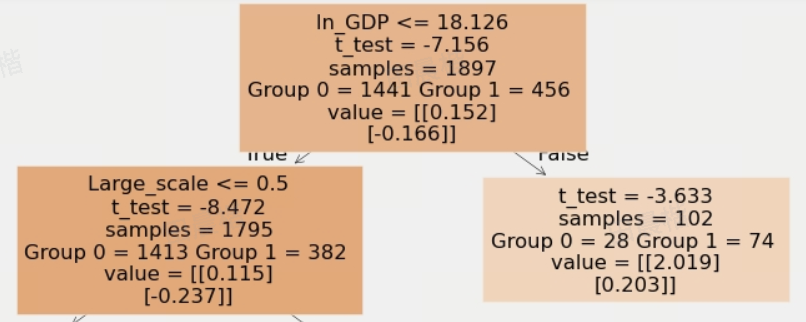
\includegraphics[width=0.8\textwidth]{Tree5.png}  
    \caption{因果树的示例单元}
    \label{fig:Tree}  
\end{figure}

我们选择区域、城市规模、行政级别、人力资本和处理前污染程度五个特征作为异质性识别目标,具体划分依据如下:

\begin{itemize}
    \item \textbf{区域差异}
    \item[$\ast$] 不同区域:根据国家统计局发布关于中国区域经济划分的官方数据。
    \item[$\ast$] 城市规模:常住人口超过300万的城市被视为大城市,而常住人口少于300万的城市则被划分为小城市。
    \item[$\ast$] 行政级别:行政地位较高的城市,如省会城市,被归为高等级城市,而其他城市则归为低等级城市。
    \item \textbf{城市特征}
    \item[$\ast$]人力资本差异:若大学生与户籍人口的平均比例高于全国平均水平,则该城市被标记为高等级;反之,则被归为低等级。
    \item[$\ast$]污染程度多样:污染排放水平高于全国平均值的城市被归为高污染城市,而低于平均值的城市则被归为低污染城市。
\end{itemize}

我们训练四棵不同参数的树,并绘制Qini图,以评估树模型的效果,。Qini图是将测试样本通过训练出来的树计算其cate,并绘制累计cate结果,Qini图下方的面积越大,表示该树的效果越好,能够区分不同特征值带来的不同影响。观察下图,横轴代表样本数,纵轴代表累计cate,此处需注意,由于PSM后的样本数发生变化,所以按照相同的训练集和测试集的比例,测试集中样本数是不同的,可以看出,经过个体层面逐年匹配处理后的数据训练出来的树模型分类效果明显好于匹配前的数据,在一定程度上说明PSM的方法是有效的。结果如图\ref{fig:Qini1}和\ref{fig:Qini2}所示:

\begin{figure}[H]
    \centering
    \caption{Qini图对比}
    \begin{subfigure}[b]{0.45\textwidth}
        \centering
        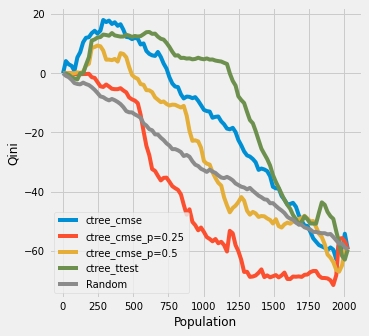
\includegraphics[width=\textwidth]{Qini1.png}
        \caption{PSM之前}
        \label{fig:Qini1}
    \end{subfigure}
    \hfill
    \begin{subfigure}[b]{0.45\textwidth}
        \centering
        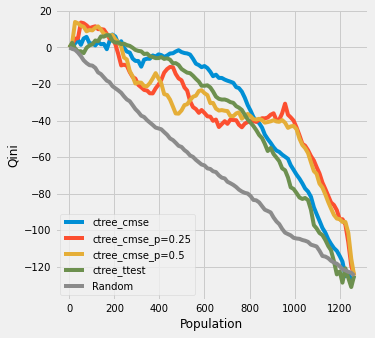
\includegraphics[width=\textwidth]{Qini2.jpg}
        \caption{PSM之后}
        \label{fig:Qini2}
    \end{subfigure}
    \label{fig:Qini}
\end{figure}

图\ref{fig:hetero}展示了异质性分析的结果。结果显示,按照异质性指标划分后的估计系数大多接近-0.5,与DDML估计结果基本一致。其中,区域特征和污染程度的异质性明显,东部城市政策效果优于西部城市,推测可能是由于东部城市政策实施效率更高、环保意识更强;高污染城市政策效果优于低污染城市,表明智慧城市建设政策在污染严重地区的环境管理方面效果显著,可能是因为这些地区污染源复杂、污染问题严重,政府和民众改善环境的意愿强烈,改进空间大。而城市规模、行政级别和人力资本三个变量的异质性不显著。

\begin{figure}[H]
    \centering
    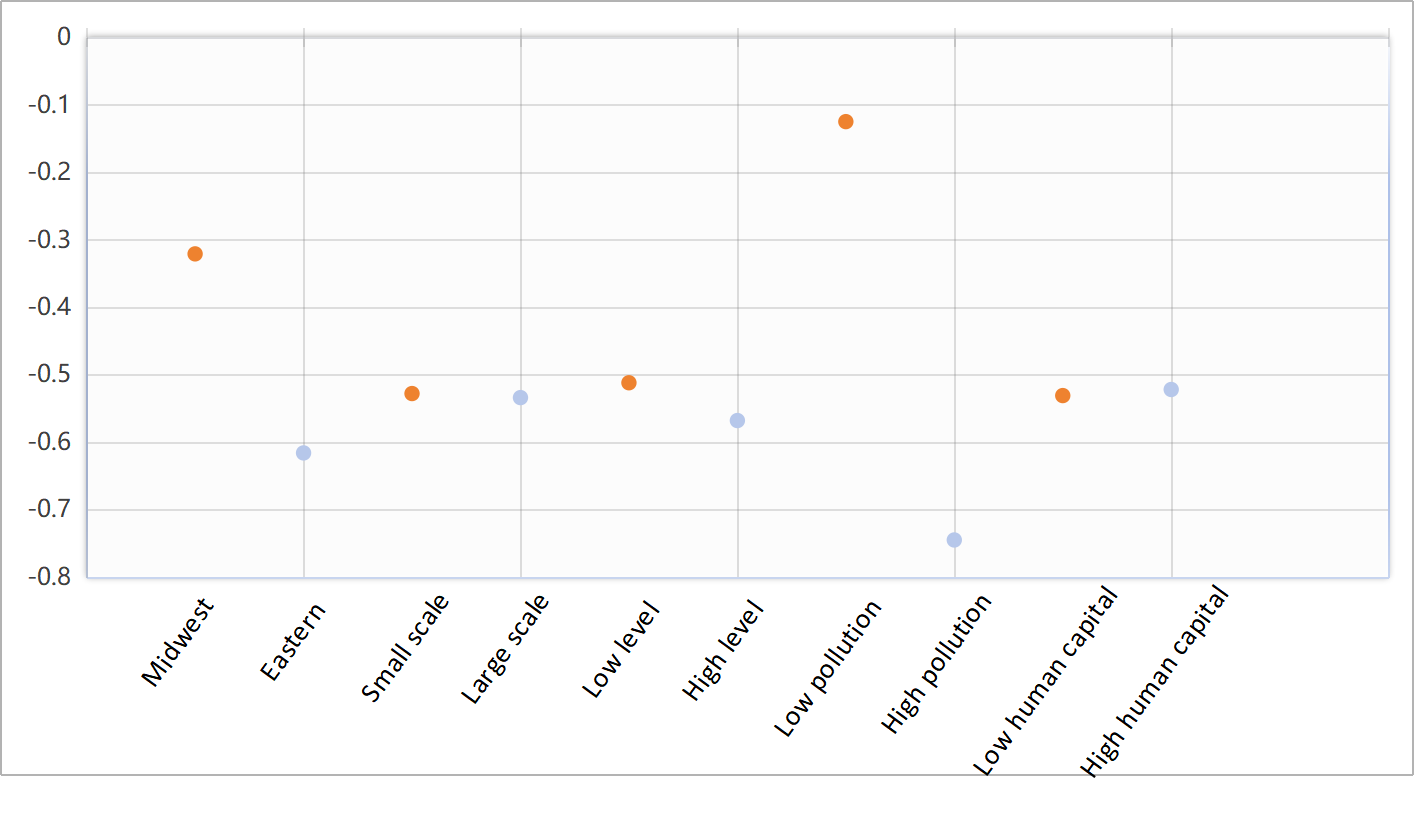
\includegraphics[width=0.8\textwidth]{Hetero.jpg}  
    \caption{异质性分析结果}
    \label{fig:hetero}  
\end{figure}


\section{贡献声明}

\begin{itemize}
    \item \textbf{田晨楷 2211333}
    \item[$\ast$] \LaTeX(幻灯片与报告)、文献研读、可视化分析、第1部分(熵权法、基准回归、Bacon 分解、平行趋势检验、安慰剂检验、PSM-DiD)的Stata实现。
\end{itemize}

\begin{itemize}
    \item \textbf{李泽宇 2212026}
    \item[$\ast$] 文献研读、可视化分析、第1部分(逐期匹配和个体层面的逐期匹配、置换因变量的稳健性检验)、第2部分(DDML、因果森林)的Python实现。
\end{itemize}

\begin{itemize}
    \item \textbf{曹涵熙 2213152}
    \item[$\ast$]文献研读、数据处理(数据获取、预处理、设置标签值)、可视化分析、报告撰写(第1部分)。
\end{itemize}

\begin{itemize}
    \item \textbf{徐乐 2212962}
    \item[$\ast$]文献研读、数据处理(数据获取、预处理、设置标签值)、可视化分析、报告撰写(第2部分)。
\end{itemize}

\newpage
\section{附录}

下面是我们小组在异质性分析中训练的四棵因果树:

\begin{figure}[H]
    \centering
    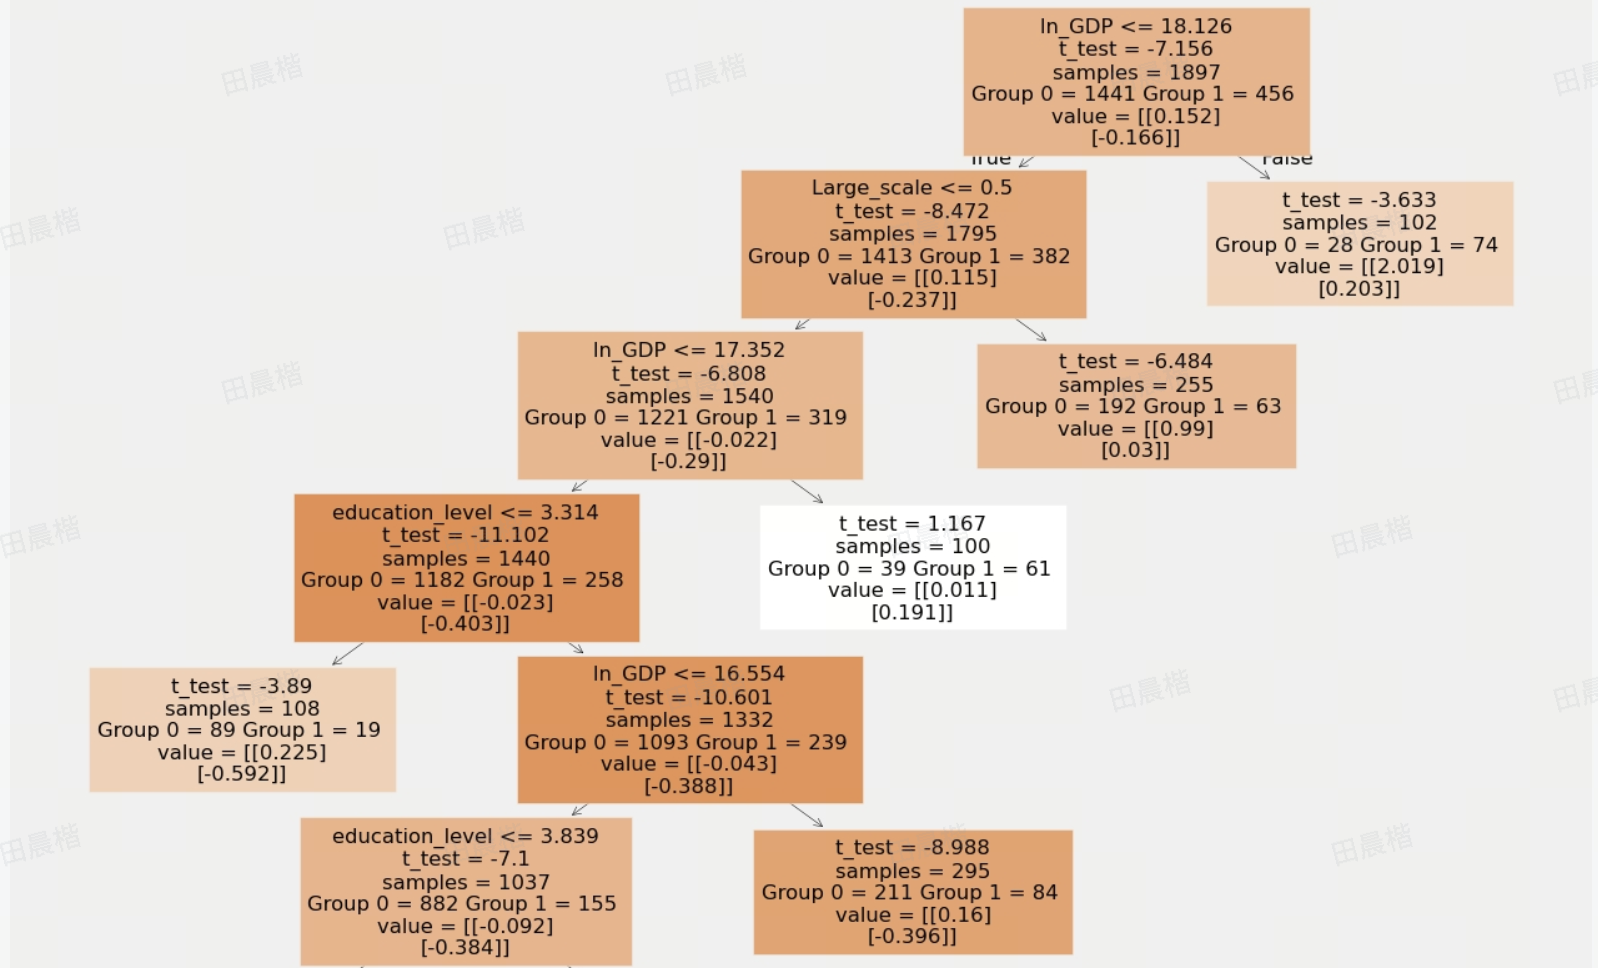
\includegraphics[width=0.8\textwidth]{Tree1.png}   
\end{figure}


\begin{figure}[H]
    \centering
    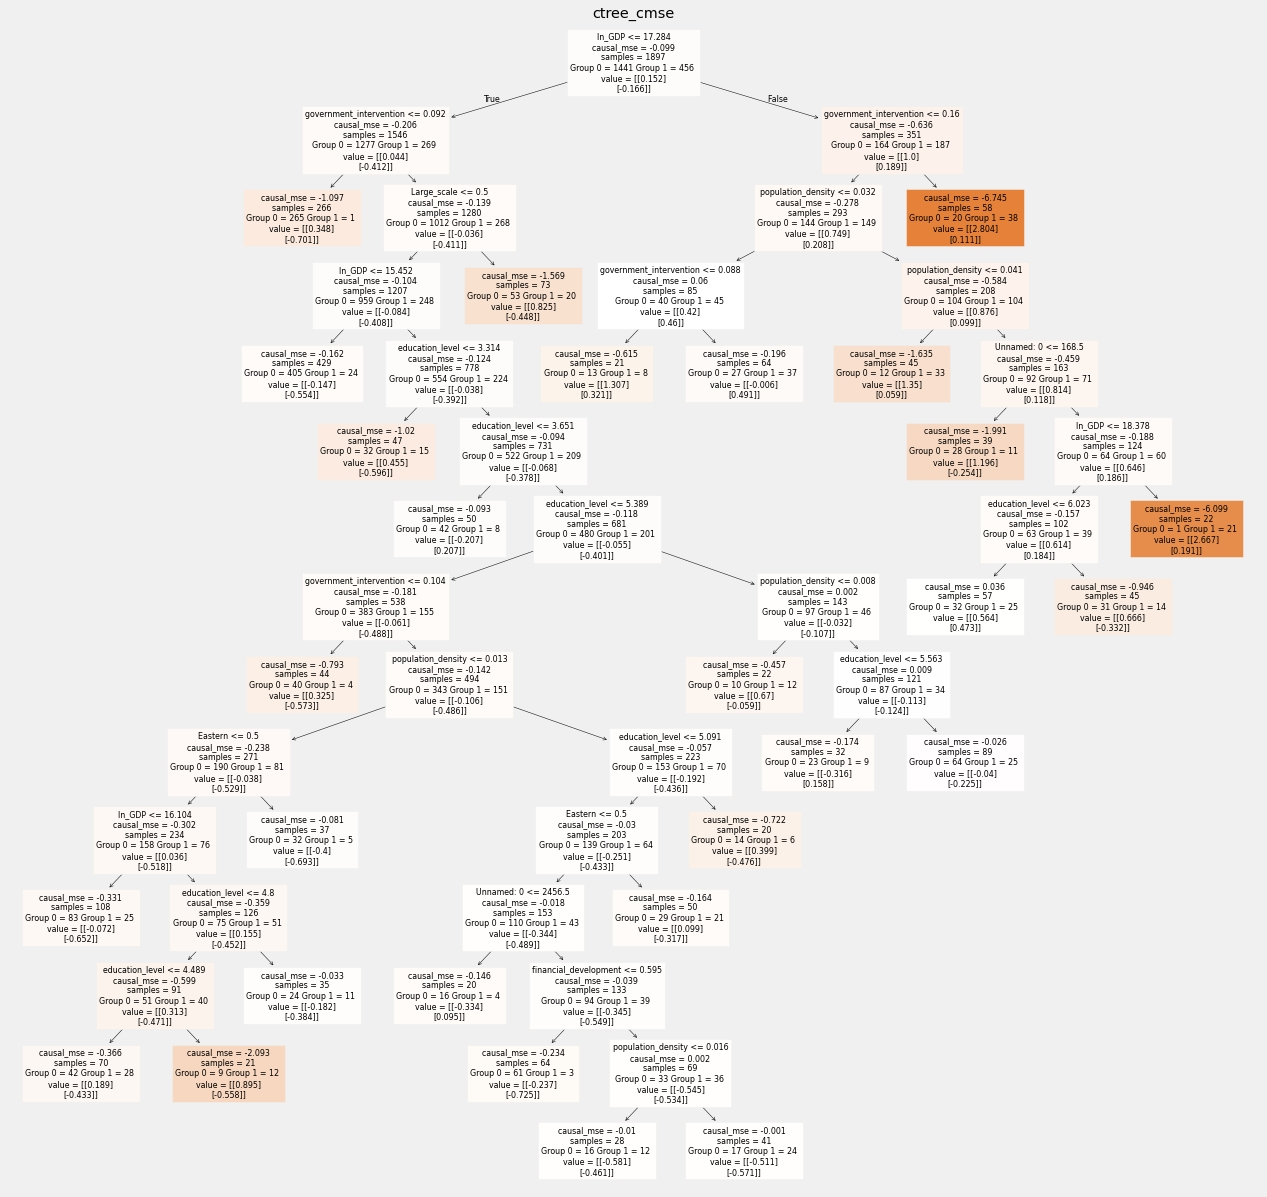
\includegraphics[width=0.8\textwidth]{Tree2.png}   
\end{figure}

\begin{figure}[H]
    \centering
    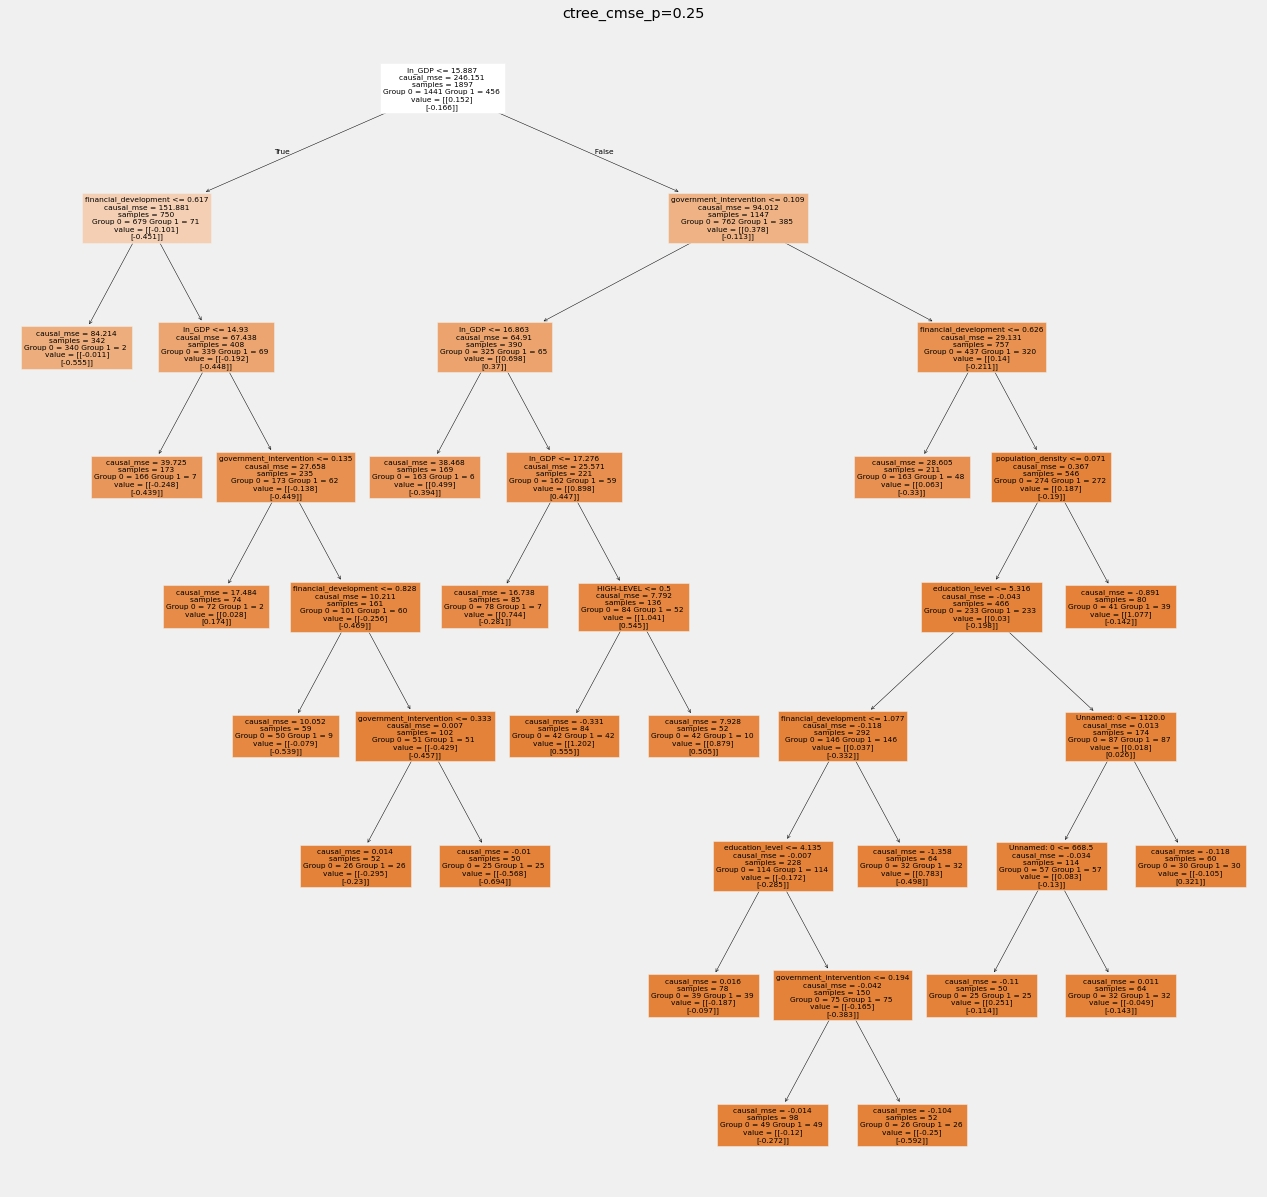
\includegraphics[width=0.7\textwidth]{Tree3.png} 
    \caption{$p=0.25$}
\end{figure}

\begin{figure}[H]
    \centering
    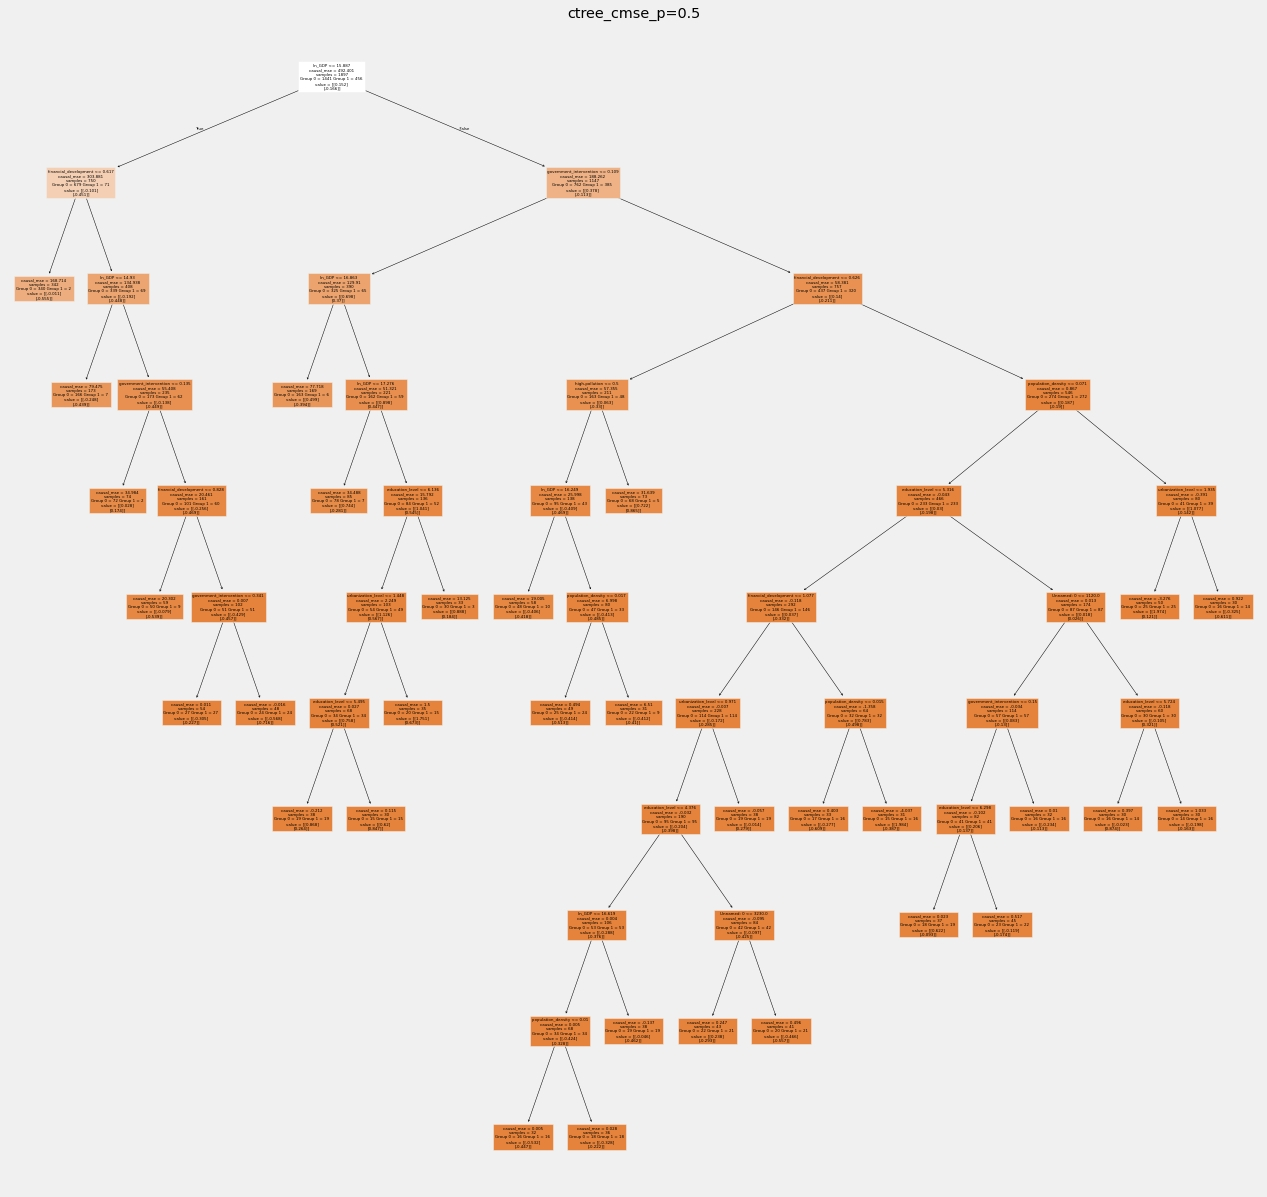
\includegraphics[width=0.7\textwidth]{Tree4.png}   
     \caption{$p=0.5$}
\end{figure}

\newpage
% 使用 \nocite{*} 包含所有参考文献
\nocite{*}

%\cite{chernozhukov2018double}\cite{farbmacher2022causal}\cite{goodman2021difference}\cite{oprescu2018orthogonal}\cite{oprescu2019orthogonal}\cite{wager2018estimation}\cite{wang2024beautifying}。

\bibliographystyle{plain} % 选择参考文献样式
\bibliography{ref} % 引用 .bib 文件

\end{document}

\subsection{}
\subsection{}
\section{}

\section{}

\section{}

\section{}
\end{document}
